\documentclass[12pt]{article}
\usepackage[utf8]{inputenc}
\usepackage{graphicx}
\usepackage[a4paper,width=150mm,top=25mm,bottom=25mm]{geometry}

\title{
{
\includegraphics[width=3cm, height=3cm]{img/LambangITS.png}}
\\
{Software Design Document for Coffee Maker}
}



\author{Author: 
\\Widian Sasi Disertasiani (5025211024) \\
Anggara Saputra (5025211241) \\
Wardatul Amalia Safitri (5025211006) \\
Muhammad Daffa’ Ashdaqfillah (5025211015) \\  
 \\ Dosen: Adhatus Solichah A., S.Kom, M.Sc}

\begin{document}

\maketitle

\section{Introduction}
\subsection{Purpose}
Dokumen desain perangkat lunak ini (SDD) menjelaskan desain arsitektur dan sistem dari aplikasi "Coffee Maker". Dokumen ini ditujukan untuk pengembang perangkat lunak, penguji, dan pemangku kepentingan lainnya yang terlibat dalam pengembangan dan pemeliharaan aplikasi ini.


\subsection{Scope}
Aplikasi "Coffee Maker" adalah sebuah sistem otomatis yang dirancang untuk menyederhanakan proses pembuatan kopi, pembayaran, dan pelaporan. Tujuan dari proyek ini adalah untuk menciptakan sebuah aplikasi yang efisien, handal, dan mudah digunakan yang dapat memenuhi kebutuhan pengguna dalam membuat kopi dengan cepat dan mudah. Manfaat dari proyek ini meliputi peningkatan efisiensi dalam proses pembuatan kopi, pengurangan kesalahan manusia, dan penyediaan laporan yang akurat mengenai transaksi dan persediaan bahan baku.

\subsection{Overview}
Dokumen ini memberikan gambaran menyeluruh tentang desain perangkat lunak aplikasi "Coffee Maker". Dokumen ini mencakup desain arsitektur, spesifikasi abstrak, desain antarmuka, desain komponen, desain struktur data, dan desain algoritma. Selain itu, dokumen ini juga membahas aspek-aspek penting seperti logging, validasi, pemantauan, dan keamanan yang diterapkan dalam aplikasi ini.

\subsection{Reference Material}
This section is optional.
List any documents, if any, which were used as sources of information for the test plan. 


\subsection{Definitions and Acronyms}
This section is optional.
Provide  definitions of all terms, acronyms, and  abbreviations that might exist to  properly 
interpret the SDD. These definitions should be items used in the SDD that are most likely not 
known to the audience.

\begin{table}[h]
\begin{tabular}{|l|l|}
\hline
\multicolumn{1}{|c|}{\textbf{Term}} & \multicolumn{1}{c|}{\textbf{Definition}}                                                                                              \\ \hline
Software Design Document (SDD)      & \begin{tabular}[c]{@{}l@{}}Digunakan sebagai media utama untuk \\mengkomunikasikan informasi desain \\ perangkat lunak.\end{tabular}                  \\ \hline
Design Entity                       & \begin{tabular}[c]{@{}l@{}}Sebuah elemen dari desain yang secara \\struktural dan fungsional berbeda dari \\ elemen lainnya.\end{tabular} \\ \hline
Service Oriented Architecture (SOA)      & \begin{tabular}[c]{@{}l@{}}Sebuah gaya arsitektur perangkat lunak \\ yang memungkinkan aplikasi untuk saling \\ berinteraksi melalui layanan yang \\ terdefinisi dengan baik..\end{tabular}                  \\ \hline
Aspect Oriented Design (AOD)        & \begin{tabular}[c]{@{}l@{}}Sebuah paradigma dalam desain perangkat \\ lunak yang bertujuan untuk meningkatkan \\ modularitas dengan memungkinkan \\ pemisahan cross-cutting concerns.\end{tabular} \\ \hline
\end{tabular}
\end{table}

\section{System Overview}
Aplikasi "Coffee Maker" adalah sebuah sistem yang dirancang untuk mengotomatiskan proses pembuatan kopi, mulai dari pemilihan menu hingga pelaporan transaksi dan persediaan bahan baku. Sistem ini terdiri dari tiga subsistem utama, yaitu Pembuatan Kopi, Pembayaran, dan Pelaporan. Subsistem Pembuatan Kopi bertanggung jawab untuk mengelola proses pembuatan kopi, termasuk pemilihan jenis kopi, pengecekan ketersediaan bahan baku, dan pembuatan kopi itu sendiri. Subsistem Pembayaran menangani proses transaksi pembayaran, termasuk penerimaan uang, pengembalian uang kembalian, dan pencatatan keuntungan. Subsistem Pelaporan bertugas menghasilkan laporan mengenai persediaan bahan baku dan keuntungan yang diperoleh dari transaksi.

\section{System Architecture}
\subsection{Architectural Design}
Arsitektur aplikasi "Coffee Maker" didasarkan pada Service Oriented Architecture (SOA) dengan strategi desain Aspect-Oriented Design (AOD). SOA memungkinkan aplikasi untuk dipecah menjadi beberapa layanan independen yang dapat saling berinteraksi. AOD memungkinkan implementasi aspek-aspek lintas fungsi seperti logging, validasi, pemantauan, dan keamanan secara terpisah dari logika bisnis utama.

Dalam arsitektur ini, terdapat tiga subsistem utama:

\begin{enumerate}
\item \textbf{Pembuatan Kopi:} Bertanggung jawab untuk mengelola proses pembuatan kopi, mulai dari pemilihan menu hingga penyediaan kopi siap minum.
\item \textbf{Pembayaran:} Menangani proses transaksi pembayaran, termasuk penerimaan uang, pengembalian uang kembalian, dan pencatatan keuntungan.
\item \textbf{Pelaporan:} Menghasilkan laporan mengenai persediaan bahan baku dan keuntungan yang diperoleh dari transaksi.
\end{enumerate}

Selain itu, terdapat juga aspek-aspek lintas fungsi yang diterapkan pada setiap subsistem:

\begin{itemize}
\item \textbf{Logging:} Mencatat setiap aktivitas yang terjadi dalam sistem, seperti pesanan yang dibuat, transaksi yang dilakukan, dan laporan yang dihasilkan.
\item \textbf{Validation:} Memastikan bahwa setiap input yang diberikan oleh pengguna valid dan sesuai dengan aturan bisnis yang berlaku.
\item \textbf{Monitoring:} Memantau kondisi sistem secara real-time, seperti ketersediaan bahan baku dan status transaksi.
\item \textbf{Security:} Melindungi sistem dari akses yang tidak sah dan memastikan keamanan data pengguna.
\end{itemize}


\begin{figure}[tbh]
\centering
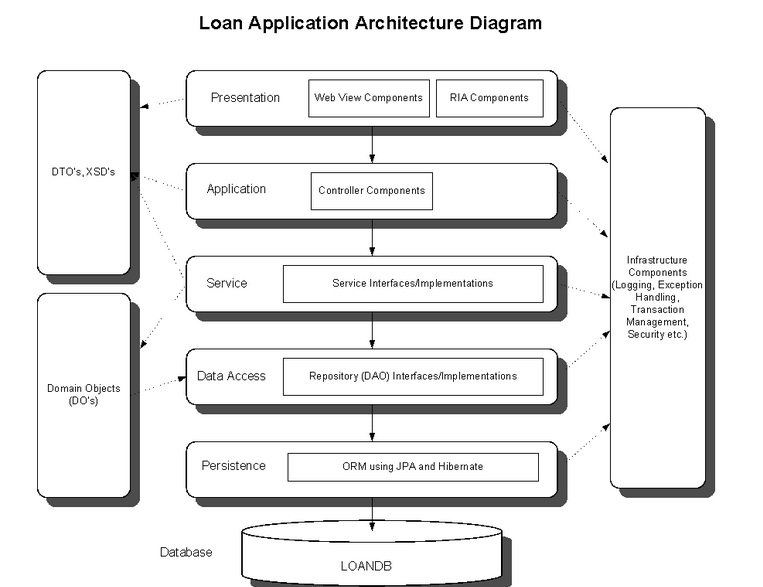
\includegraphics[width=0.7\linewidth]{./img/image}
\caption{Architectural Design}
\label{fig:image}
\end{figure}


\subsection{Decomposition Description}
Desain komponen yang terdapat dalam aplikasi "Coffee Maker" dibagi menjadi tiga subsistem utama, yaitu Pembuatan Kopi, Pembayaran, dan Pelaporan.

\begin{itemize}
\item \textbf{Pembuatan Kopi:} Terdapat tiga jenis kopi yang berbeda, yaitu Espresso, Latte, dan Cappuccino. Setiap objek kopi memiliki variabel untuk menyimpan informasi mengenai jumlah air (water), kopi (coffee), susu (milk), dan harga (price). Method \texttt{makeCoffee()} digunakan untuk mengurangi stok bahan baku dan menambahkan harga kopi ke total pembelian.    
\item \textbf{Pembayaran:} Terdapat empat jenis koin yang dapat diterima oleh aplikasi, yaitu Penny, Nickel, Dime, dan Quarter. Setiap objek koin memiliki variabel untuk menyimpan nilai nominal dari koin tersebut. Method \texttt{insertCoin()} digunakan untuk memasukkan koin ke dalam mesin, dan method \texttt{returnChange()} digunakan untuk memberikan kembalian kepada pengguna jika pembayaran melebihi harga minuman.
\item \textbf{Pelaporan:} Terdapat dua jenis laporan, yaitu laporan stok bahan baku dan laporan penjualan. Method \texttt{generateStockReport()} digunakan untuk menghasilkan laporan stok bahan baku, dan method \texttt{generateSalesReport()} digunakan untuk menghasilkan laporan penjualan.
\end{itemize}

    

Struktur data yang digunakan dalam aplikasi "Coffee Maker" meliputi:
\begin{itemize}
\item Array/List: Digunakan untuk menyimpan daftar jenis kopi yang tersedia, serta daftar atribut dari setiap jenis kopi seperti water, coffee, milk, dan price.
\item Dictionary or Map: Digunakan untuk menyimpan nilai nominal koin (Penny, Nickel, Dime, dan Quarter) dalam bentuk pasangan key-value.
\item Object/Classes: Digunakan untuk merepresentasikan entitas subsistem seperti pembuatan kopi, pembayaran, dan pelaporan.
\end{itemize}

\subsection{Design Rationale}
Arsitektur SOA dipilih karena kemampuannya untuk memecah aplikasi menjadi layanan-layanan independen yang dapat dikembangkan, diuji, dan dikelola secara terpisah. Hal ini memudahkan dalam pengembangan dan pemeliharaan aplikasi, terutama dalam tim yang besar. Selain itu, SOA juga memungkinkan skalabilitas yang lebih baik, karena setiap layanan dapat ditingkatkan secara independen sesuai kebutuhan.

Strategi desain AOD dipilih karena kemampuannya untuk mengimplementasikan aspek-aspek lintas fungsi secara terpisah dari logika bisnis utama. Hal ini meningkatkan modularitas dan reusabilitas kode, karena aspek-aspek tersebut dapat diterapkan pada berbagai bagian aplikasi tanpa harus mengubah kode utama. Selain itu, AOD juga memudahkan dalam pemeliharaan dan pengembangan aplikasi, karena perubahan pada aspek-aspek tersebut dapat dilakukan tanpa mempengaruhi bagian lain dari aplikasi.


\section{Data Design}
\subsection{Data Description}
Aplikasi "Coffee Maker" akan menyimpan berbagai jenis data untuk mendukung operasionalnya:

\begin{itemize}
\item \textbf{Data Bahan Baku:} Informasi mengenai jumlah air (dalam mililiter), susu (dalam mililiter), dan kopi bubuk (dalam gram) yang tersedia di dalam mesin akan disimpan dan diperbarui secara berkala.
\item \textbf{Data Harga Kopi:} Harga untuk setiap jenis kopi, yaitu Espresso, Latte, dan Cappuccino (dalam dolar), akan disimpan dalam sistem.
\item \textbf{Data Koin yang Dimasukkan:} Jumlah masing-masing jenis koin yang dimasukkan oleh pengguna, seperti Quarters (25 sen), Dimes (10 sen), Nickels (5 sen), dan Pennies (1 sen), akan dicatat untuk keperluan pembayaran dan perhitungan kembalian.
\end{itemize}

\section{Data Dictionary}
Berikut adalah daftar entitas sistem atau data utama dalam aplikasi "Coffee Maker" beserta tipe dan deskripsinya:

\begin{tabular}{|l|l|p{10cm}|}
\hline
\textbf{Entitas} & \textbf{Tipe} & \textbf{Deskripsi} \\
\hline
Coffee & Object & Merepresentasikan jenis kopi (Espresso, Latte, Cappuccino) dengan atribut water, coffee, milk, dan price. \\
\hline
Coin & Object & Merepresentasikan jenis koin (Penny, Nickel, Dime, Quarter) dengan atribut value. \\
\hline
Inventory & Object & Menyimpan informasi mengenai persediaan bahan baku (air, kopi, susu) dengan atribut masing-masing dan uang dalam mesin (money). \\
\hline
Transaction & Object & Merepresentasikan sebuah transaksi dengan atribut coffeeType, payment, dan change. \\
\hline
StockReport & Object & Merepresentasikan laporan stok bahan baku dengan atribut water, coffee, dan milk. \\
\hline
SalesReport & Object & Merepresentasikan laporan penjualan dengan atribut totalSales dan totalProfit. \\
\hline
CoffeeMachine & Object & Merepresentasikan mesin kopi dengan method-method untuk membuat kopi (makeCoffee), menerima pembayaran (insertCoin), memberikan kembalian (returnChange), dan menghasilkan laporan (generateStockReport, generateSalesReport). \\
\hline
UserInterface & Object & Merepresentasikan antarmuka pengguna untuk berinteraksi dengan mesin kopi. \\
\hline
\end{tabular}

\section{Component Design}
Desain komponen aplikasi "Coffee Maker" dibagi menjadi tiga subsistem utama, yaitu Pembuatan Kopi, Pembayaran, dan Pelaporan. Berikut adalah penjelasan lebih rinci mengenai masing-masing komponen:

\begin{enumerate}
    \item \textbf{Pembuatan Kopi (Coffee)}
    \begin{itemize}
        \item \textbf{Atribut:}
        \begin{itemize}
            \item water (int): Jumlah air yang dibutuhkan (dalam ml).
            \item coffee (int): Jumlah kopi yang dibutuhkan (dalam gram).
            \item milk (int): Jumlah susu yang dibutuhkan (dalam ml).
            \item price (float): Harga kopi.
        \end{itemize}
        \item \textbf{Method:}
        \begin{itemize}
            \item makeCoffee(): Mengurangi stok bahan baku sesuai dengan jenis kopi yang dipilih dan menambahkan harga kopi ke total pembelian.
        \end{itemize}
    \end{itemize}


    \item \textbf{Pembayaran (Coin)}
    \begin{itemize}
        \item \textbf{Atribut:}
        \begin{itemize}
            \item value (float): Nilai nominal koin.
        \end{itemize}
        \item \textbf{Method:}
        \begin{itemize}
            \item insertCoin(): Memasukkan koin ke dalam mesin, memperbarui jumlah total uang yang dimasukkan, dan mengembalikan objek Transaction.
            \item returnChange(): Menghitung dan mengembalikan kembalian kepada pengguna jika ada.
        \end{itemize}
    \end{itemize}

    \item \textbf{Pelaporan (StockReport, SalesReport)}
    \begin{itemize}
        \item \textbf{Atribut:}
        \begin{itemize}
            \item StockReport.water (int): Jumlah air tersisa.
            \item StockReport.coffee (int): Jumlah kopi tersisa.
            \item StockReport.milk (int): Jumlah susu tersisa.
            \item SalesReport.totalSales (float): Total penjualan.
            \item SalesReport.totalProfit (float): Total keuntungan.
        \end{itemize}
        \item \textbf{Method:}
        \begin{itemize}
            \item generateStockReport(): Menghasilkan laporan stok bahan baku.
            \item generateSalesReport(): Menghasilkan laporan penjualan.
        \end{itemize}
    \end{itemize}
\end{enumerate}

\paragraph{Algoritma Design (Pseudocode):}

\subparagraph{app.py}
\begin{verbatim}
Import pembuatanKopi.py, pembayaran.py, pelaporan.py

makeCoffee()
insertCoin()
returnChange()
generateStockReport()
generateSalesReport()
\end{verbatim}

\subparagraph{pembuatanKopi.py}
\begin{verbatim}
def makeCoffee():
    input -> coffeeType
    logCoffee(coffeeType)
    monitorCoffee(coffeeType)
    validateCoffee(coffeeType)
\end{verbatim}

\subparagraph{pembayaran.py}
\begin{verbatim}
def insertCoin():
    input -> coinAmount

def returnChange():
    logPayment(coinAmount)
    monitorPayment(coinAmount)
    validatePayment(coinAmount)
    securePayment(coinAmount)
\end{verbatim}

\subparagraph{pelaporan.py}
\begin{verbatim}
def generateStockReport():
    logReport(stock)
    securePayment(stock)

def generateSalesReport():
    logReport(sales)
    securePayment(sales)
\end{verbatim}

\subparagraph{monitoring.py}
\begin{verbatim}
From logging.py import Menu, Resources

def monitorCoffee(coffeeType):
    # Monitoring logic for coffee making
    For item in coffeeType.ingredients:
        Resources[amount] -= coffeeType.ingredients[item]

def monitorPayment(paymentAmount, coinType):
    for coin in Coin_values:
        money_received += paymentAmount * coinType[currency]
    return money_received
\end{verbatim}

\subparagraph{security.py}
\begin{verbatim}
def securePayment(paymentAmount):
    # Security measures for payment handling
    If != authority person:
        Return false
    Return 0

def secureReport(reportType):
    # Security measures for report generation
    If != authority person:
        Return false
    Return 0
\end{verbatim}

\subparagraph{validation.py}
\begin{verbatim}
From logging.py import Menu, Resources

def validateCoffee(coffeeType):
    # Validation logic for coffee type
    if coffeeType not in ["latte", "espresso", "cappuccino"]:
        Return false
    For item in coffeeType.ingredients:
        If Resources[amount] < coffeeType.ingredients[item]:
            Return false
    Return 0

def validatePayment(paymentAmount):
    # Validation logic for payment amount
    if paymentAmount <= 0:
        Return false
    If paymentAmount < totalPayment:
        Return false
    Return 0
\end{verbatim}

\subparagraph{logging.py}
\begin{verbatim}
Menu = [MenuItem(name, water, milk, coffee, cost)]
Resources = {ingredients: amount}
Coin_values = {coin: currency}
Profit = 0

def logCoffee(coffeeType):
    add new item into Menu

def logPayment(paymentAmount):
    add new coin into coin_values

def logReport(reportType):
    if Type == sales:
        print(profit)
    elif Type == stock:
        print(resources)
\end{verbatim}


\section{Human Interface Design}

\subsection {Overview of User Interface}
Describe the functionality of the system from the user s perspective. Explain  how the user 
will be  able  to use  your system to complete  al the  expected  features and  the  feedback 
information that will be displayed for the user.

\subsection {Screen Images}
Display screenshots showing the interface from the users perspective. These can be  hand drawn
or you can use an automated drawing tool. Just make them as accurate as possible.



\subsection {Screen Objects and Actions}
A discussion of screen objects and actions associated with those objects.


\section{Requirements Matrix}
Provide a cross reference that traces components and data structures to the requirements in your
SRS document.
Use  a  tabular  format to show  which system  components satisfy each of the  functional 
requirements from the SRS. Refer to the functional requirements by the numbers/codes that you 
gave them in the SRS.


\section{APPENDICES}
This section is optional.
Appendices may be included, either directly or by reference, to provide supporting details that could 
aid in the understanding of the Software Design Document.

\section {References}
\bibliographystyle{IEEEtranS}

\bibliography{bab/dissertationbib}

\end{document}
